\chapter{Topology in non-Hermitian systems}
\label{ch:nh}
In quantum mechanics, the condition that the observable must be a Hermitian operator has a deep physical reasoning - the corresponding expectation value has to be a real-valued number. However, this strong assumption can be relaxed - it is possible to have a non-Hermitian operator with real spectrum. This observation gave rise to the concept of PT-symmetric Hamiltonians, where the real spectrum is guaranteed by the product of parity and time-reversal symmetries~\cite{BenderPT1998}.

Another motivation comes from the open systems. Instead of a full treatment with Lindblad formalism, for instance, nH Hamiltonians can effectively capture the coupling of the system with its environment, where the non-Hermiticity models the gains and losses.

Such system exhibits interesting phenomena without Hermitian counterpart: exceptional points, the skin effect and, as a consequence, the breakdown of bulk-boundary correspondence.

Novel features of nH systems are seen at the level of $2 \times 2$ matrices. Consider a matrix M:
M = \begin{equation}
\begin{pmatrix}
0 & \alpha \\
1 & 0 
\end{pmatrix}
\end{equation}


If $\alpha \neq 1$, $M$ is not diagonalizable, and only admits the Jordan block form. NH matrices have distinct left- and right- eigenvectors. Therefore, a remedy for some problems may be to consider quantities of interests within the biorthogonal quantum mechanics. For instance, the norm is then given by the inner product between left and right eigenvectors. This attempt allowed to restore BB correspondence in some models. Another way is to consider the singular value decomposition (SVD) instead of eigenvalue problem. However, the interpretation of the singular values is not physical (in contrast to the eigendecomposition, where the eigenvalues are the energies)~\cite{SVDHerviou2019}.




In non-Hermitian case, the topology is already manifested in single-band systems (in contrast to Hermitian systems where at least two bands are needed). Also, the winding number for 1D systems is defined through the eigenvalues, not the eigenstates.


\section{Exceptional points}
Let us remind the concept of Weyl points. Consider the Hamiltonian in 3D
\begin{equation}
H =\mathbf{k} \cdot \boldsymbol{\sigma} = k_x \sigma_x + k_y \sigma_y + k_z \sigma_z.
\label{eq:weylh}
\end{equation}
This model exhibits a robust generic degeneracy. As all $\sigma_i$ are used, adding other term proportional to $\sigma_i$ only shifts the touching point. Now compare the following model in 2D:
\begin{equation}
H = k_x \sigma_x + k_y \sigma_y + i r \sigma_y
\label{eq:excepth}
\end{equation}
Non-zero $r$ gives rise to  the degeneracies in non-Hermitian band structure called exceptional points. Exceptional points can be seen as equivalents of Weyl nodes as they appear in generic points in $k$-space and one has to get them closer to annhilate them (for example by adding very large mass term).

\begin{figure}
\centering
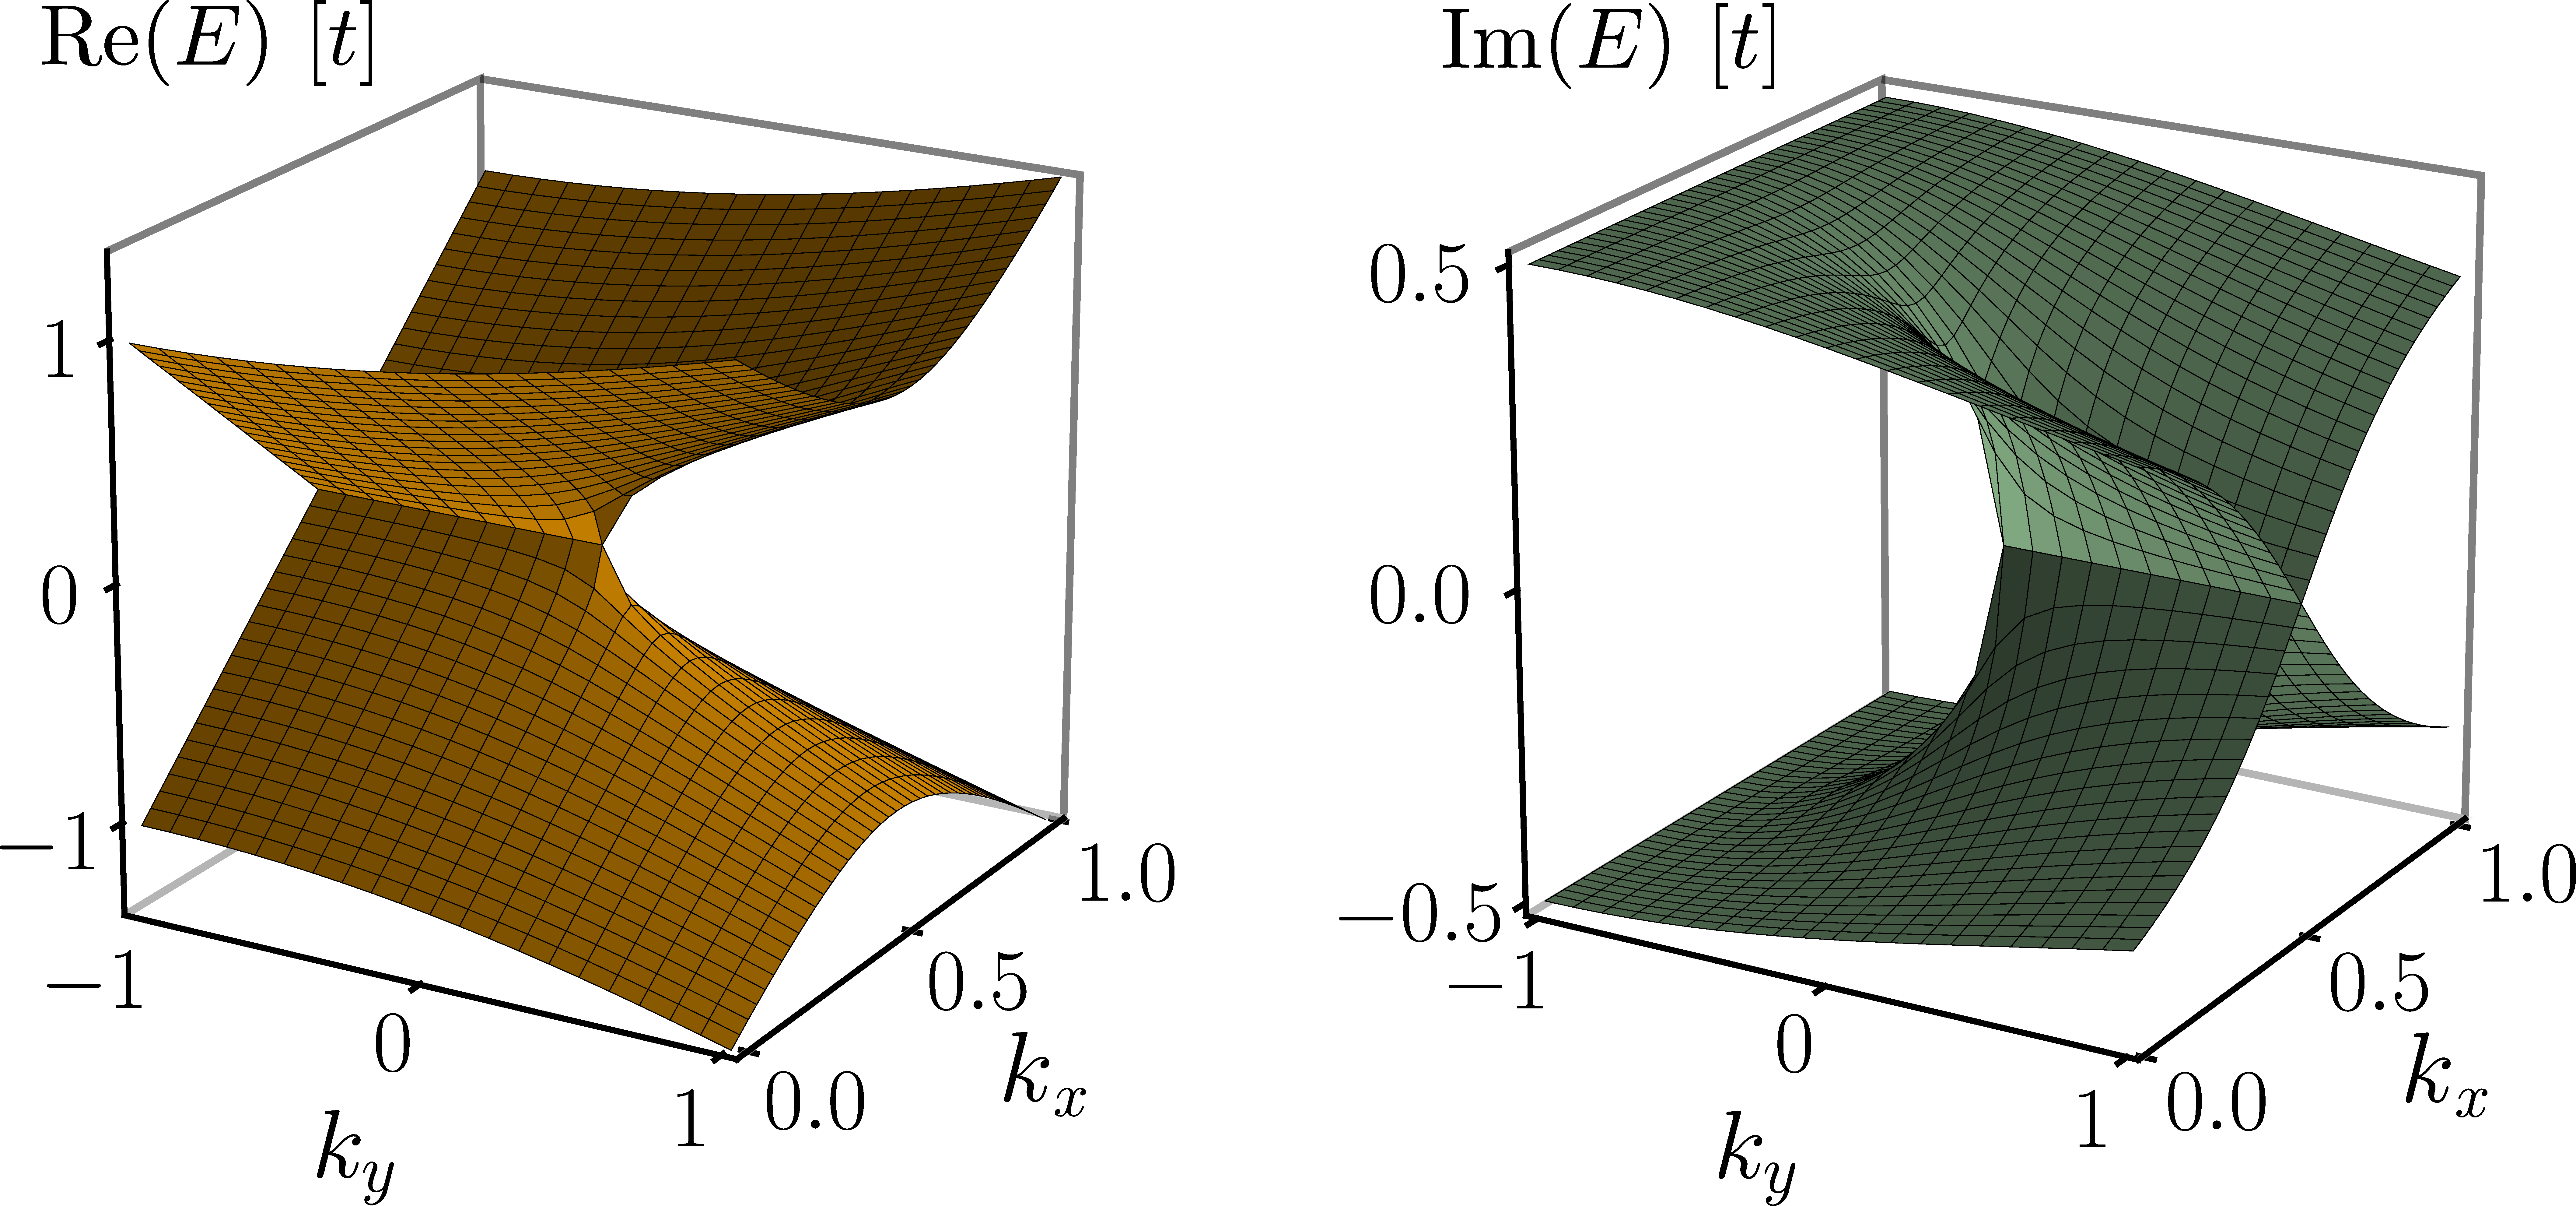
\includegraphics[width=\columnwidth]{nh_exceptional.pdf}
\caption{Real (left) and imaginary (right) part of the spectrum of the Hamiltonian defined by Eq.\eqref{eq:excepth}. Gapless region of real part of the spectrum corresponds to gapped imaginary spectrum and vice versa.}
\label{fig:excepth}
\end{figure}



\section{Breakdown of bulk-boundary correspondence}


As Hermitian conjugate is not longer equal to complex conjugate and transpose, different type of symmetries appear. Classification, firstly by~\cite{Bernard_2002}, extended recently in Refs.~\cite{PhysRevLett.120.146402, PhysRevX.8.031079, PhysRevB.99.125103}



\section{Skin effect}
nH Hamiltonians are sensitive to the boundary conditions. Eigenstates localization properties may change dramatically. All states for the system in an open geometry may be exponentially localized on the one edge, which is dubbed the skin effect (note: this has nothing in common with a typical skin effect, where the electrons in a conductor prefer to flow far from the middle due to electron-electron repulsion).

Previously, it was known that the skin effect can be induced by having unbalanced directed hoppings. However, this breaks the reciprocity, defined as 
\begin{equation}
H (k) = H^{T} (-k)
\label{eq:recipSE}
\end{equation}


\subsection{Reciprocal skin effect}

Here, we show that in two- or higher-dimensions it is possible to have the skin effect with the condition defined by Eq.~\eqref{eq:recipSE}.

